\section{Switch String}

O \textit{Switch with String} veio no Java 7 e trouxe este recurso que porém pequeno é efetivamente útil porque ajuda a escrever o código mas legível e além do mais o compilador 
irá gerar o \textit{codebyte} com mais eficiência em comparação com \textit{if-then-else}. Nos projetos analisados foram somente encontrados 77 oportunidades de migração para \textit{switch with string}.

\begin{figure}[h]
	\center
	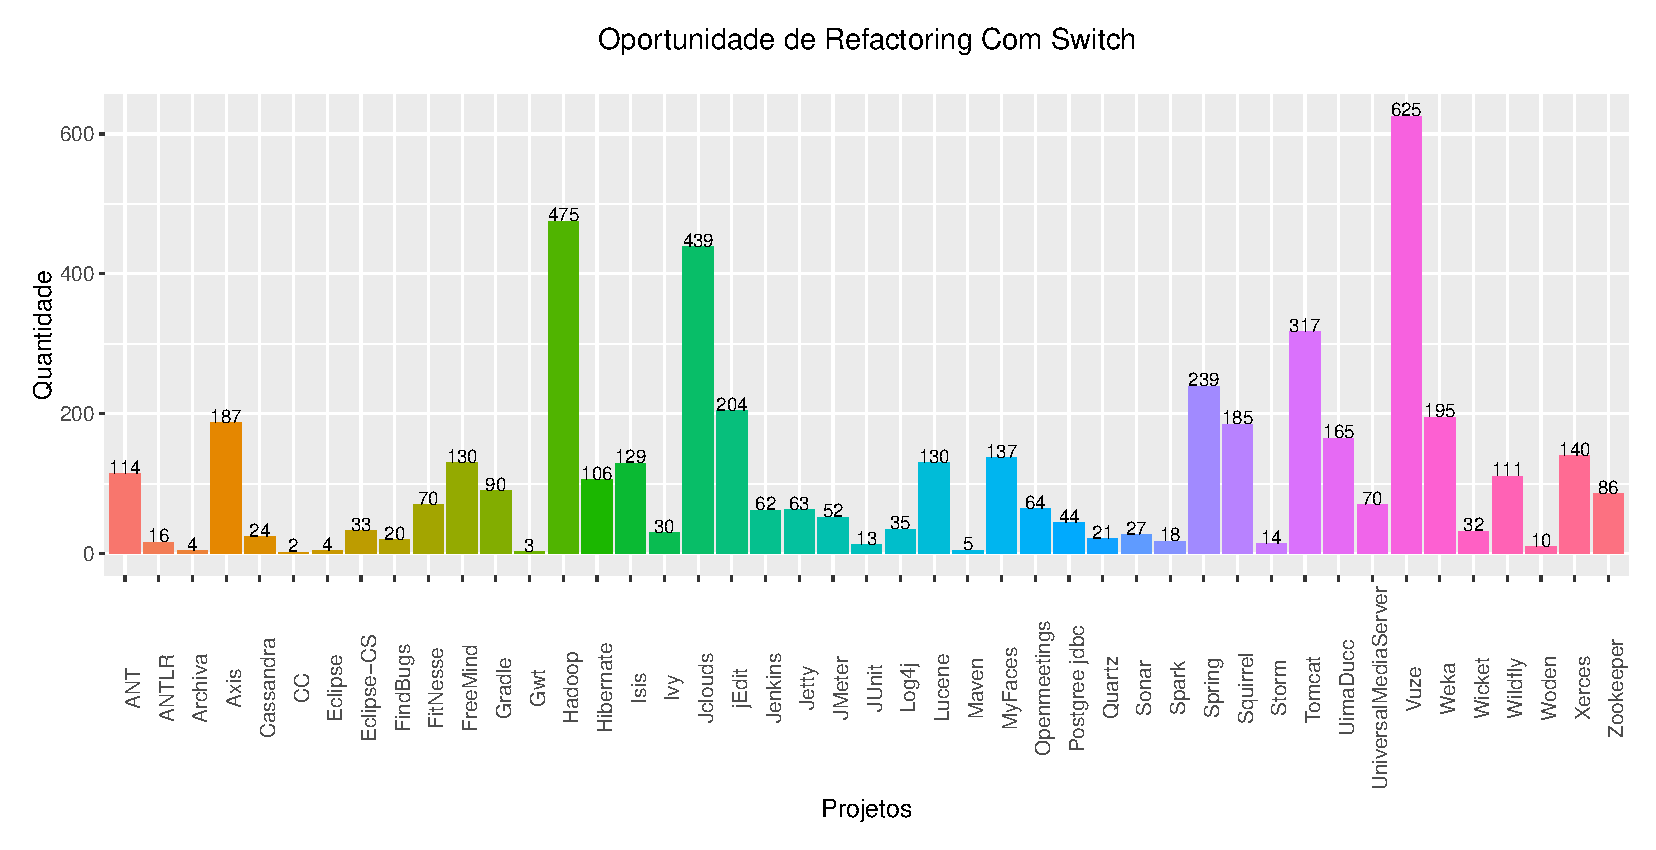
\includegraphics[scale=0.5]{Imagens/oportunidadesSwitchString}
	\label{fig:Switch with String}
	\caption{Oportunidades de \textit{Switch with String} nos projetos.}
\end{figure}

Conforme exibido na imagem acima das diferentemente do \textit{switch with string} o uso desse recurso seria mais bem empregado no projeto o \textit{Weka} pois teria uma redução de 31 \textit{if - else} anhinhados comparando \textit{Strings} onde seria mais elegante a evolução sem grande impacto pois teria um código mais elegante e atual.
